\documentclass[a4paper,spanish,11pt,twoside]{article}
\usepackage[spanish]{babel}
\usepackage[utf8]{inputenc}
\usepackage{verbatim}
\usepackage{fancyhdr}
\usepackage{lmodern}
%\usepackage{url}
\usepackage{anysize}

\usepackage[T1]{fontenc}
\usepackage[bookmarks,hyperfootnotes=false,colorlinks=true,urlcolor=black,linkcolor=black,citecolor=black,pagecolor=black,anchorcolor=black,breaklinks=true]{hyperref}% Hiperenlaces

\usepackage{graphicx}
\usepackage{fixme}
\graphicspath{{figures/}}

% Párrafos
\setlength{\parskip}{8pt}
%interlineado

\marginsize {35mm}{20mm}{25mm}{25mm}

\renewcommand{\baselinestretch}{1.5}
\begin{document}


\renewcommand*{\thepage}{\roman{page}}
\begin{titlepage}
\begin{center}
  
\includegraphics[width=.3\textwidth]{logos/emblema_informatica-gray.pdf} \\
  \vspace*{0,5cm} {\Large \textsc{Universidad de Castilla-la Mancha\\}}
  \vspace{3mm}
  {\Large \textbf{Escuela Superior de Informática}}  \\
  \vspace{1,3cm}
  {\Large \textbf{Ingeniería en Informática}}\\
  \vspace{1cm}
  {\Large \textbf{Work Diary}} \\
  \vspace{1,3cm}
  \LARGE{\textbf{Geo-Cloud}\\Modelling and Implementation of the Geo-Cloud Experiment for the Fed4FIRE European Project}
  %\vspace{0.1cm}

\end{center}
\vspace{1.0cm}
\begin{table}[!h]
  \Large
  \begin{tabular}{rl}
      \textbf{Autor}: & Rubén Pérez Pascual \\
      \textbf{Director}: & Jonathan Becedas Rodríguez \\
      \textbf{Tutor}: & Carlos González Morcillo
  \end{tabular}
\end{table}
% \vspace{1,5cm} \\
\begin{flushright}
%\vspace{1cm}
{\large \today}
\end{flushright}
\end{titlepage}




\newpage
\thispagestyle{empty}
\tableofcontents
\newpage

\pagestyle{fancy}
\fancyhead[L]{Diary of work}
\fancyhead[R]{Rubén Pérez Pascual}
\fancyfoot[C]{\thepage}
\renewcommand{\sectionmark}[1]{\markboth{\textbf{\thesection. #1}}{}}
\renewcommand*{\thepage}{\arabic{page}}
 \setcounter{page}{1}



%\section{Introducción}
\chapter{Introduction}

\drop{E}{arth} Observation (EO) commercial data sales have increased a 550\% in
the last decade \cite{sousa}[1]. This area is considered a key element in the
space industry and an opportunity market for the next years.

\ac{EO} industries implement on-premises conventional infrastructures to acquire,
store, process and distribute the geo-information generated.

However these solutions have the risks of over/under size the infrastructure, they are not flexible to cover sudden changes in the demand of services and the access to the information presents large latencies.  These aspects limit the use of \ac{EO} technology for real time use such as to manage crises, natural disasters and civil security among others (Deren, 2007).

In addition, new sectors and user typologies are applying for new \ac{EO} services
and there is an incresing demand of this services. These users
need more flexible, easy and instant access to \ac{EO} products and services through
the Web. This demand has traditionally been driven through Space Data
Infrastructures and heavy standards (ISO TC/211 and OGC) which are focused on
interoperability rather than the real demand from the end-users.

The use of cloud computing technology can overcome the previously defined limitations that present conventional infrastructures because of its elasticity, scalability and on-demand use characteristics (Armbrust, 2010).

GEO-Cloud Experiment goes beyond conventional data infrastructures used in \ac{EO}
industry and beyond the implementations of applications running in cloud, to
quest which parts of a complete infrastructure of \ac{EO} are technologically and
economically viable to be virtualized to offer basic and high added value
services (see Figure~\ref{fig:intr-geocloudConcept}).

\begin{figure}[!h]
\begin{center}
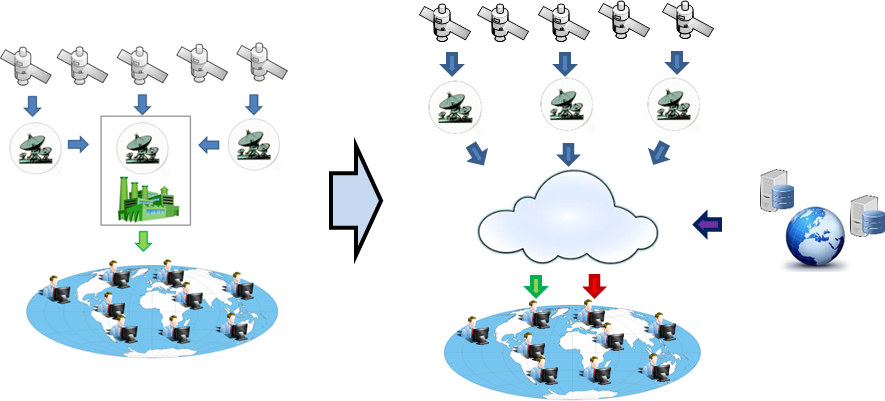
\includegraphics[width=0.6\textwidth]{statement/geocloudConcept.png}
\caption{The GEO-Cloud Concept. It is based on the use of cloud technology to acquire data, store it, process it, integrate it with other sources and distribute it to end users with the final objective of testing viable solutions for its real implementation.}
\label{fig:intr-geocloudConcept}
\end{center}
\end{figure}

GEO-Cloud  emulate the remote sensing mission with the satellites, the
topology network and the communications in the \vw testbed. The data
acquired from the emulated satellites is transferred to the \bonfire cloud
for storage, processing and distribution of data. End users accessing and
broadcasting will be emulated in another network implemented in \vw. In
order to implement realistic impairments in \vw, real networks will be
tested in \pl.  The technologies for imagery distribution and \ac{EO}
service delivery using cloud technologies and Internet protocols will be tested.

\section{Earth Observation}


\section{Cloud Computing}


\section{The Fed4FIRE European Project}


\section{The Geo-Cloud Experiment Overview}


\subsection{Experiment Description}

The experiment consists of virtualizing a conventional \ac{EO} system to offer on
demand services to clients with the objective of validating its viability, find
the strengths and weaknesses of using cloud computing technology and establish
possible solutions for a future implementation in the market. There are three
components:
\begin{enumerate}
\item \emph{In-orbit mission:} this component generates the raw data. This consists of un-processed images of the Earth captured by a constellation of satellites and downloaded to different ground stations.
\item \emph{Treatment of data:} the data has to be stored, processed at different levels based on the services offered and distributed to the clients. The data acquired by the in-orbit mission is integrated with other sources to provide higher quality services.
\item \emph{End-users:} users of the provided services with different levels of remote access rights.

\end{enumerate}


\subsubsection{Experiment Design}


The GEO-Cloud experiment requires emulating a complete realistic Earth Observation Mission to provide high added value services such as crisis management. To this complex situation, the system has to response by processing on demand massive and variable amounts of stored and on line transferred data.

GEO-Cloud makes use of the following \emph{Fed4FIRE} facilities: \pl,\vw and
\bonfire. \pl allows us to measure real network characteristics geographically
distributed to setup our models. \vw allows us to create any desired network
topology and emulate the in-orbit mission and the web service to the
users. \bonfire provides us a real cloud infrastructure with observability in
all the layers to test our cloud based services.


\paragraph{Implementation of the acquisition of geo-data in Virtual Wall and
  PlanetLab}~\\
The acquisition of geo-data is obtained from the in-orbit mission. The
constellation of satellites and the ground stations are emulated in \vw. A
network topology is implemented to communicate the different satellites with the ground stations. Every satellite in its orbit and every ground station models are simulated in a node.

The satellite models simulate the orbits and the pass of the satellites over the ground stations. The ground stations models simulate the coverture of the antennas and the download of the data. When a satellite is inside this radius, the satellite downloads the data to the ground station that is visible. The downloaded data in the ground stations is transferred to the \bonfire cloud.

With the \vw network,the \emph{bandwidths, latencies and loss rates} are
controlled.Also a realistic network topology to transfer data between different
nodes is created.

In order to determine the correct link characteristics for the connections
between the ground and the cloud infrastructure, a profilling tool has been
developed for measuring appropriate values for the link impairment between these different geographical locations using the \pl testbed.


\paragraph{Implementation of the cloud based services in BonFIRE}~\\
To facilitate offering the previous services we propose to implement a multi-layered cloud model in the \bonfire cloud infrastructure to generate on demand geo-information. The multi-layered cloud model is constituted of two layers:
\begin{itemize}
\item \emph{Layer 1:} This layer involves the basic satellite imagery services.  It acquires the raw data, stores it, has the first level of processing, distributes the processed data and offers the hosting service.

\item \emph{Layer 2:} This layer involves the high added value services. It can use historical processed, real time captured and pre-processed data from layer 1. This layer processes the information for real time generation of geo-information and offers real time access and distribution to the end-users. Typically, the implementation of high added value EO services involves the ingestion of the raster imagery from the satellites into a spatial database or storage, where it can be refined, simplified, processed or combined with other data sources in vector or raster format. The products, which can be vector or raster data, are distributed or queried using Internet technologies (OGC standards like WMS) or through Web services (tiles, caches, etcetera).
\end{itemize}

Thus, the whole EO system is completely implemented in Fed4FIRE, see Figure 3.

\begin{figure}[!h]
\begin{center}
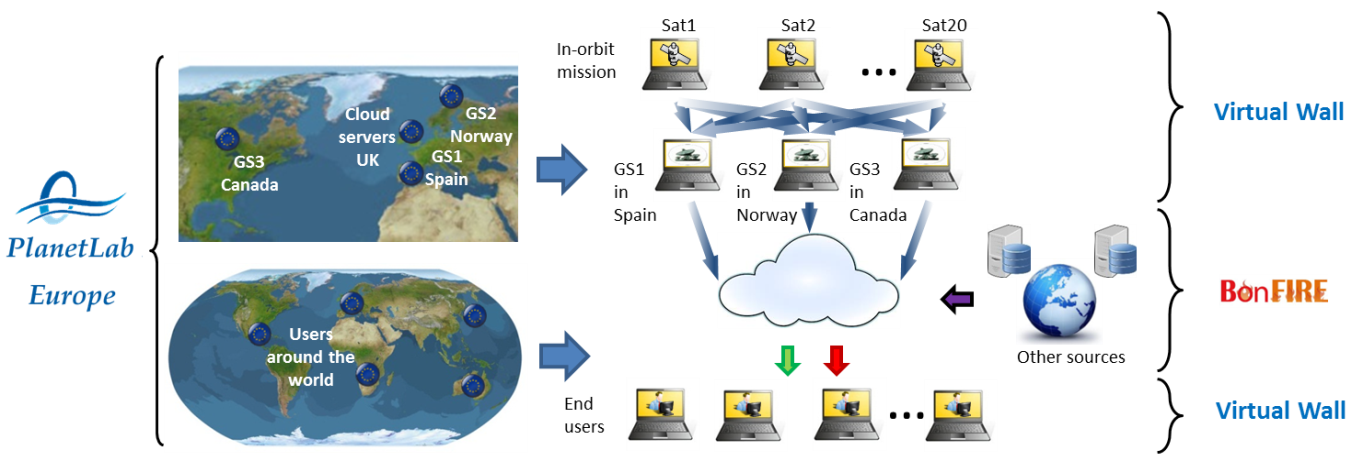
\includegraphics[width=0.6\textwidth]{statement/testbeds-geocloud.png}
\caption{Geo-Cloud implementation in Fed4FIRE}
\label{fig:intr-testbeds-geocloud}
\end{center}
\end{figure}




\subsection{Impact in Fed4FIRE}
The experiment will contribute to several objectives of the \emph{Fed4FIRE} project:
increase trustworthiness of its facilities and support their
sustainability. GEO-Cloud will test \emph{Fed4FIRE} tools for its use in the industry
driven experiments close to market, specifically complex and real time services
for Earth Observation industry when critical situations occur. 
GEO-Cloud will validate the tools for monitoring and control of cloud computing
and networking in EO services for emergencies and will test the limits of the
infrastructure for processing, storing and traffic of massive on-demand
data. GEO-Cloud will provide feedback to improve the infrastructure during and
after the experiment is carried out, sharing our knowledge in traditional
infrastructures for \ac{EO} applications, monitoring, processing and
distribution of geospatial data.

\subsection{Scientific and Technological Impact}

GEO-Cloud will contribute to provide a worldwide service in the Earth
Observation Industry. It will answer if Future Internet technologies can provide
viable solutions for the complex \ac{EO} market and to find the limitations of
the current cloud computing technology for its application in \ac{EO} market.
 
GEO-Cloud will test the viability and ease of use of those facilities for
industry driven experiments close to the market.

\subsection{Socio-Economical Impact}

The Geo-Cloud project is used as a framework to offer services from \ac{EO}
users. The benchmark developed in the experiment allows to establish the
frontiers of viable and not viable cloud solutions in \ac{EO} depending on the
type of demand and service offered. This will establish the basis to satisfy the
growing demand of added value \ac{EO} services.

The reduction of the processing, sotrage, communications and distribution costs
of {EO} services will facilitate the access to the remote sensing techonology of
common end users, but also of a more general public. GEO-Cloud will contribute
defining the basis to advance in the use of geospatial information of the nine
``Societal Benefit Areas'' defined in GEO: disasters, health, energy, climate,
water, weather, ecosystems, agriculture and biodiversity; by demonstrating
whether or not cloud computing offers technologically and economically viable
solutions to offer highly demanding services.

The results obtained in the experiment will be used by our company to offer new
services to th general public, current end users and future potential users. The
rest of the \ac{EO} industry will be beneficiated since we will define a
benchmark that relates the demand with the technology to offer quality
services. The users will be beneficiated since we will define the framework to
offer higher quality services.




\section{Document Structure}

This document has been carried out as the end of carrier project rules from the \emph{Escuela
Superior de Informática} of the \emph{Universidad de Castilla La Mancha}. It contains
the following sections:


\begin{definitionlist}
\item[Chapter \ref{chap:antecedentes}: \nameref{chap:antecedentes}] in this
  chapter an overview of the necessary knowledge areas is made to study for the
  development of GEO-Cloud, like cloud computing, distributed middlewares,
  processing premises for \ac{EO} and several testbeds in Fed4FIRE.
\item[Chapter \ref{chap:objetivos}: \nameref{chap:objetivos}] in this
  chapter, the main objectives are depicted and explained for GEO-Cloud.
\item[Chapter \ref{chap:method}: \nameref{chap:method}] in this chapter the
  selected metodology is explained and justified. Also, the uses resources such
  Fed4FIRE's testbeds, hardware and software are depicted.
\item[Chapter \ref{chap:arquitectura}: \nameref{chap:arquitectura}] TODO
\item[Chapter \ref{chap:antecedentes}: \nameref{chap:antecedentes}] Explica herramientas
  y aspectos básicos de edición con \LaTeX.
\item[Capítulo \ref{chap:objetivos}: \nameref{chap:objetivos}] Finalidad y justificación
  (con todo detalle) del presente documento.
\end{definitionlist}


%\section{Objetivos}
%objetivos.tex

\section{Objetivos}
\label{sec:objetivos}

Según lo expuesto en la sección \ref{sec:intro}, sería deseable disponer de
un sistema que simule una constelación de satélites y varias estaciones de tierra con sus respectivas métricas en las comunicaciones. Además, que el procesado de los datos en bruto obtenidos en las estaciones de tierra se realice en la nube y la adquisición de esas imágenes procesadas por parte de los clientes sea real.

\begin{figure}
\begin{center}
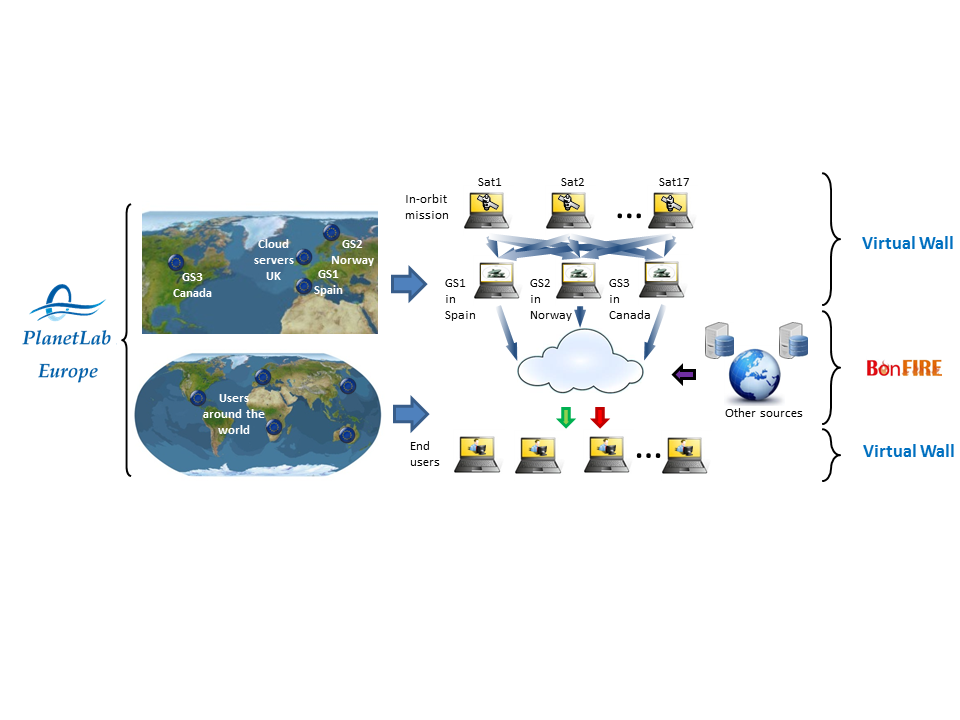
\includegraphics[width=.9\textwidth]{GEOCloud_in_Fed4FIRE.png}
\caption{Geo-Cloud en Fed4FIRE}
\end{center}
\end{figure}

Por ello en este proyecto se plantean los siguientes objetivos:

\begin{itemize}

\item \textbf{Implementación de los servicios basados en Cloud en la plataforma BonFIRE:}  Se pretende desarrollar un servicio de procesamiento de datos Raw y creación de orto-imágenes en Cloud. Para esta implementación será necesario conocer la arquitectura de la cadena de procesado que se implementa en Elecnor Deimos. Además se debe de dar soporte a las peticiones de los clientes con lo cuál se deben de implementar servicios de distribución de estos resultados entre los usuarios finales.

\item \textbf{Implementación de la constelación de satélites, estaciones de tierra y clientes sobre PlanetLab Europe:}Otro aspecto a tener en cuenta serían las métricas. Para esto se usará PlanetLab Europe, con la que conseguiremos simular conexiones de red entre distintos nodos distribuidos por el mundo.
A tavés de la implementación del modelo de red en PlanetLab Europe se podrán medir las características de una red real. Se realizarán dos capas en esta implementación. La primera modelará las estaciones de tierra y la constelación; la segunda, los clientes finales accediendo a los servicios Cloud.

\item \textbf{Implementación de la constelación de satélites, estaciones de tierra y clientes sobre VirtualWall:} Tras realizar la implementación sobre PlanetLab Europe, se conseguirá toda la información de una red real, con lo que se realizará un modelo sobre VirtualWall de acuerdo a esos parámetros. Además esta plataforma permitirá tener completo control sobre los recursos y todos los factores envueltos en los distintos casos de prueba, con lo que se podrá evaluar su comportamiento.

\item \textbf{Simulación de distintos escenarios y obtención de resultados:} Tras realizar la implementación de lo anteriormente expuesto, se procederá a realizar uno o varios casos de prueba con los que obtengamos datos para contrastar como actúa este servicio de procesado de obtención de geo-imágenes en la nube frente a la misma implementación sobre un centro de procesamiento de datos.



\end{itemize}







% Local Variables:
%   coding: utf-8
%   fill-column: 90
%   mode: flyspell
%   ispell-local-dictionary: "castellano"
%   mode: latex
%   TeX-master: "main"
% End:



\clearpage
% \section{Licencia}
% \input{licencia.tex}


 \bibliography{references}
  \bibliographystyle{plain}

\end{document}
